\chapter{Evaluation}
 In this chapter it is shown the steps for implementing the MFW, the evaluation score that will be use for testing it and the results of testing it under different conditions.
 
 \section{Algorithm}
 
The MWF noise reduction method was implemented in Matlab following these steps:

\begin{enumerate}
\item Compute the auto and cross $PSD$ of both inputs.
\item Find the single microphone SPP $\rho$ and noise PSD with \eqref{SPP} or \eqref{SPPyong} and \eqref{psdNoi}
\item Apply a single channel noise reduction method to the reference. 
\item Obtain correlation matrices with \eqref{corrv} and \eqref{corry}.
\item Obtain the estimated matrix $\hat{\textbf{r}}_{yx}$ with \eqref{requ} using the filtered reference of step 3.
\item Obtain filter  $\textbf{W}_{MWF_\lambda}$  with \eqref{mwfeq}.
\item Obtain $Z$ as $Z(k,n)=\textbf{W}_{MWF_\lambda}^H(k,n)\textbf{y}(k,n)$.
\end{enumerate}

The MWF was implemented in Matlab with both previously showed SPP algorithms and with both methods to avoid stagnation. Here it will be shown how to evaluate the performance of this implementation and the results of it.

\section{Data Base}

To test in the most accurately possible way all the noise reduction methods, it is necessary to have a proper data base and a proper algorithm to run the measurement metric. For this is was used a radio studio with 4 microphones, one main speaker and a set of several speakers.

The data base consists of 10 voices (5 female and 5 male) and 5 different kind of usual noises.

The main speaker and microphones were arranged as shown in figure \ref{fig:DataB} where $D=50cm$ and $d=10cm$. The main speaker was reproducing the clean voice files and the set of speakers was placed all around the studio to create a good simulation of  spatially homogeneous distributed noise.



\begin{figure}[!ht]
  \centering
	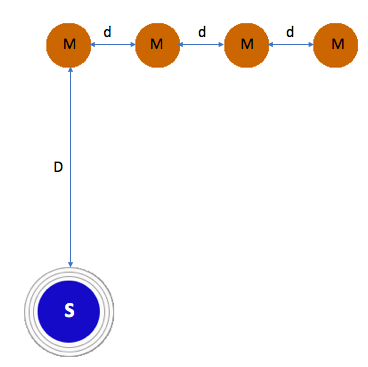
\includegraphics[width=120mm]{Kap4/DataB}
	\caption{Microphone array and audio source positions.}
	\label{fig:DataB}
\end{figure}

\section{Perceptual Evaluation of Speech Quality}

As shown in \cite{Sharma2014AMeasure}, the measure of PESQ (Perceptual Evaluation of Speech Quality) is a measure which evaluates the similarity between two speech signals in a perceptual scale. This means that a high value of PESQ means a good speech enhancement method.

The score of PESQ is given in dBs, where the higher score means better speech enhancement.

The Matlab code capable of performing the PESQ evaluation between two signals was taken from \cite{Loizou}. 

In order to obtain accurate scores, two files from the voice data base were taken (one female voice and one male voice) and two from the noise database and each voice was mixed with each noise in a range of SNR of $[-30dB , 15dB]$. These signals were taken as imputs for the different filters, and then the output of each filter was plotted and compared with the other methods and with the original noisy signal. 


\section{Results}

The results of the evaluation process are shown in figures \ref{fig:female3n}, \ref{fig:male3N}, \ref{fig:female2n}, \ref{fig:MaleN1}. The method labeled as "Gerk" refers to the one found in \cite{Gerkmann2011NoisePresence} and the one labeled as "Yong" refers to the one found in \cite{SPPYONG} and the label "Noisy" is the noisy input with no filter. The use of these methods with each of the algorithms to avoid stagnation and their combination were plotted and their PESQ score is displayed. \\






\begin{figure}[!ht]
  \centering
	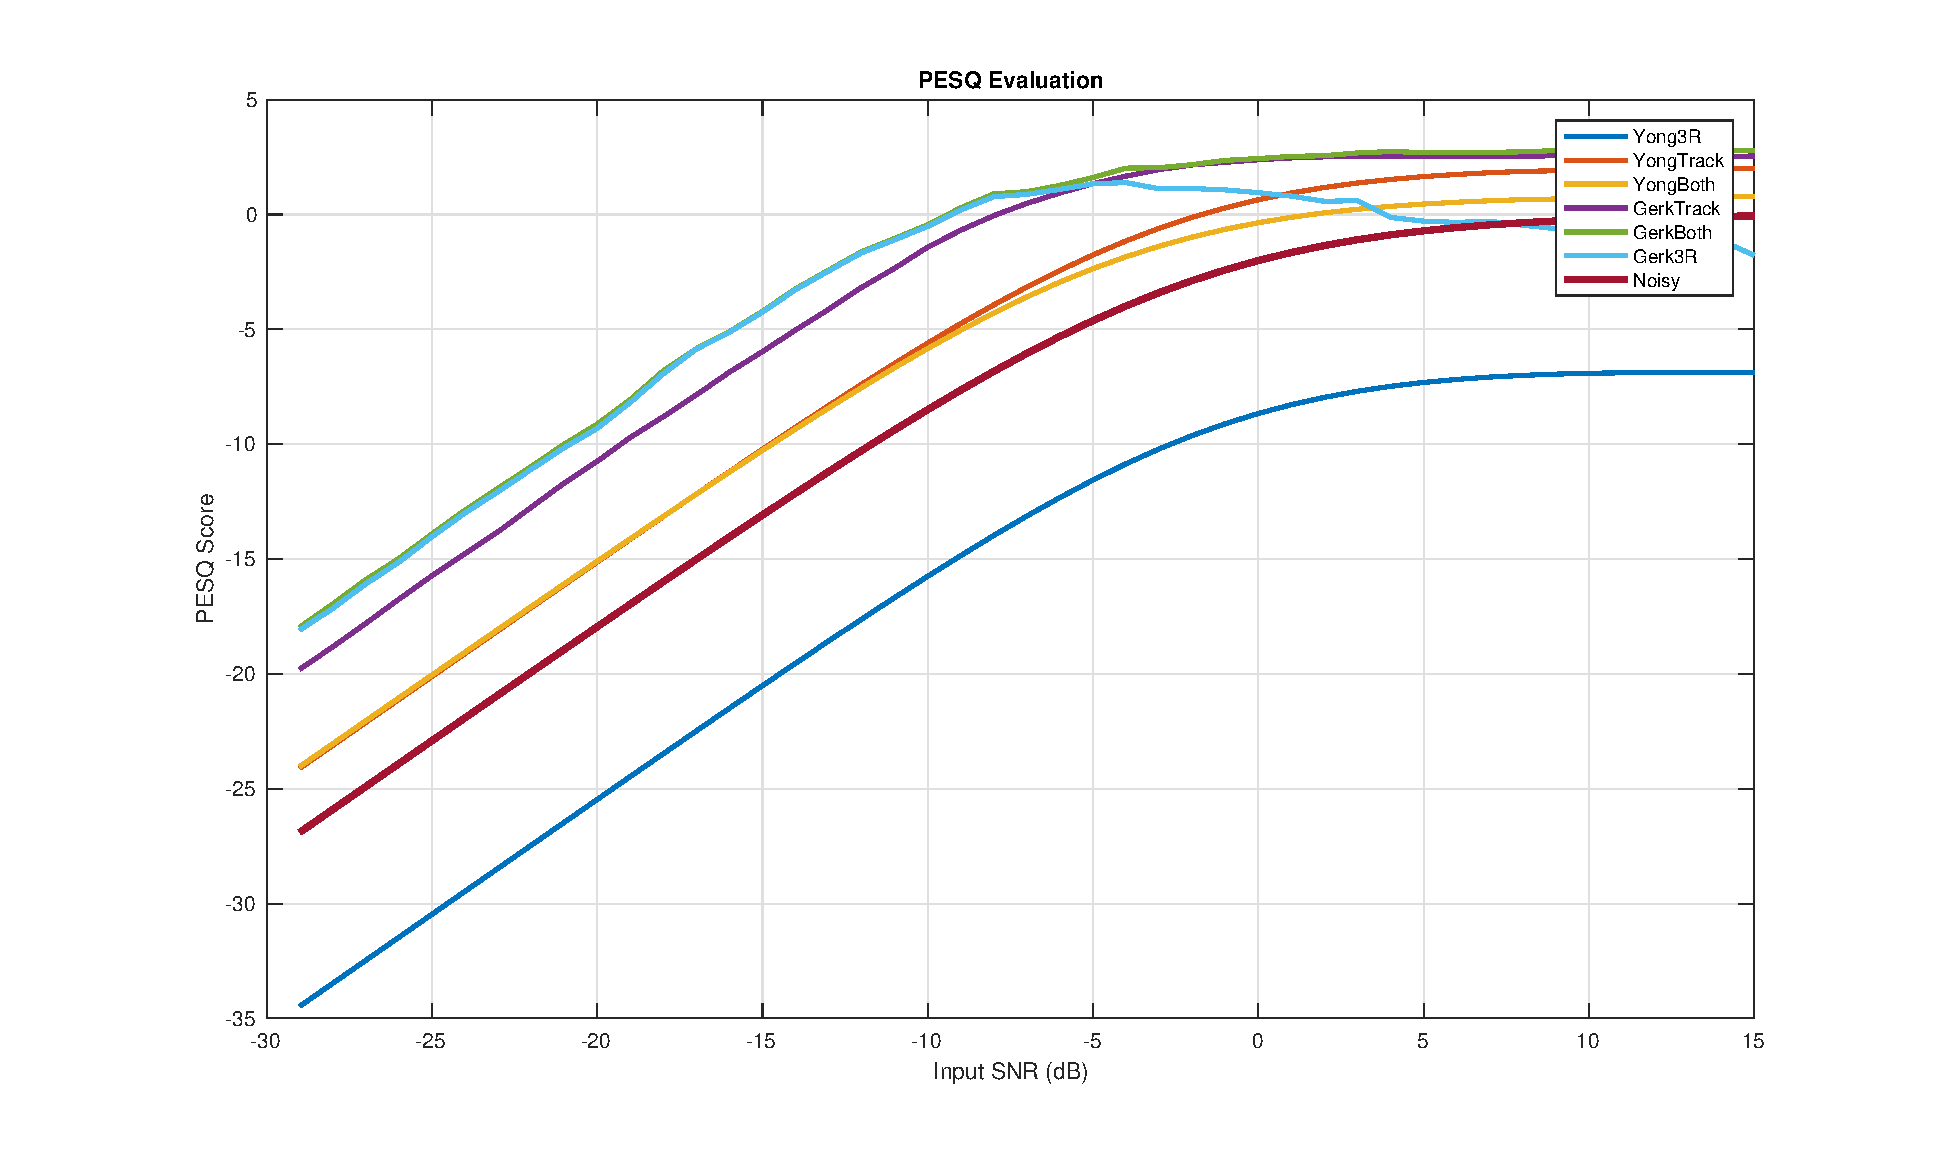
\includegraphics[width=130mm]{Kap4/female3n}
	\caption{PESQ results for female voice and car noise audios.}
	\label{fig:female3n}
\end{figure}

It can be seen in all figures that the combination of "Yong" with the 3 regions method leads to an important voice degradation and its PESQ values are always lower than the noisy input, however when this method is used with the tracking time algorithm, the score increases and there is speech enhancement. This can be caused by the speed in which this method updates the SPP value not being compatible with the 3 regions. In this case, combining both algorithms for avoiding stagnation doesn't improve the value. \\

\begin{figure}[!ht]
  \centering
	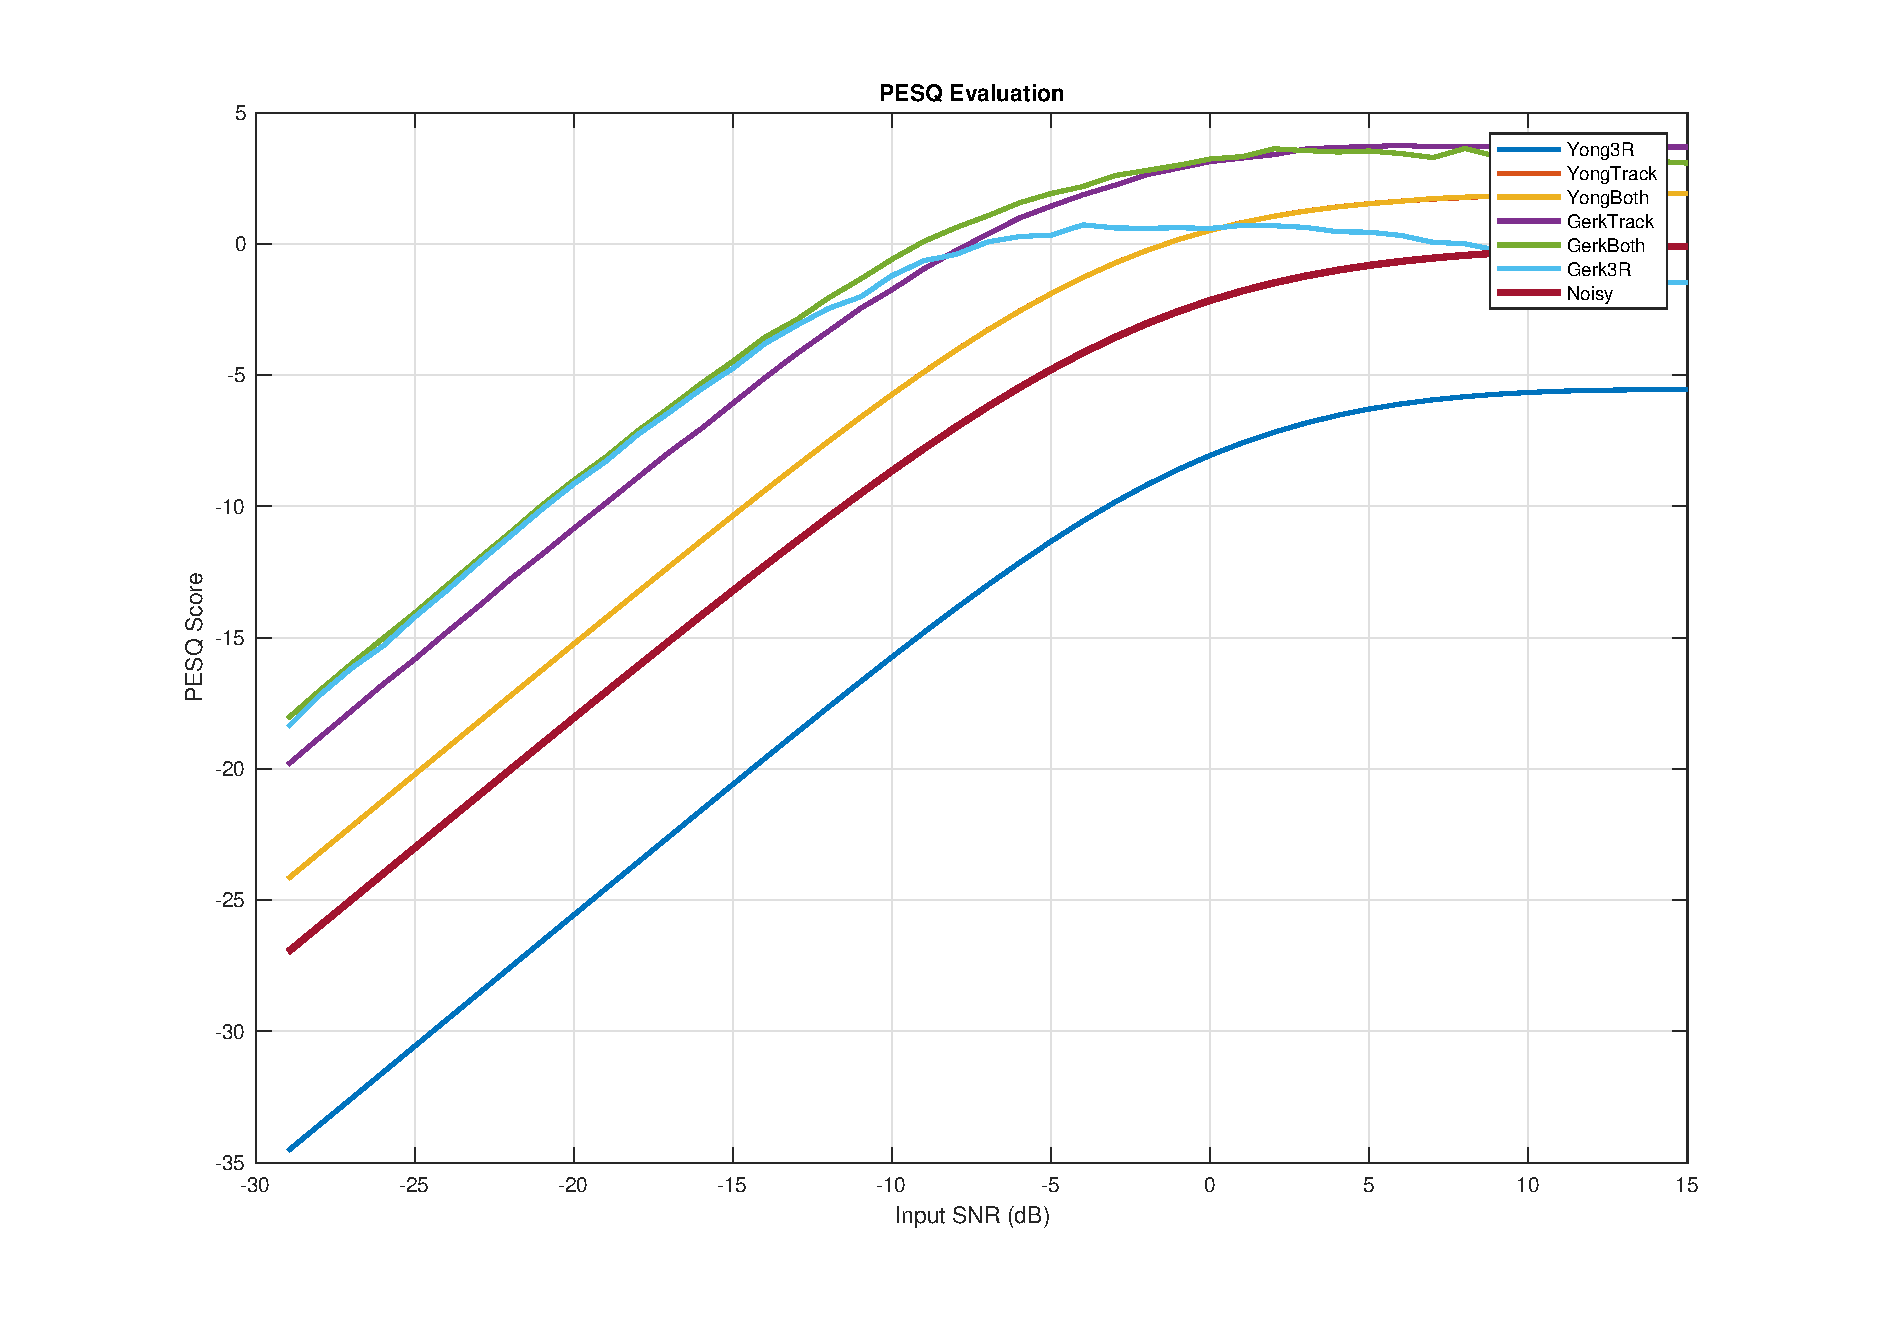
\includegraphics[width=130mm]{Kap4/male3N}
	\caption{PESQ results for male voice and car noise audios.}
	\label{fig:male3N}
\end{figure}


\begin{figure}[!ht]
  \centering
	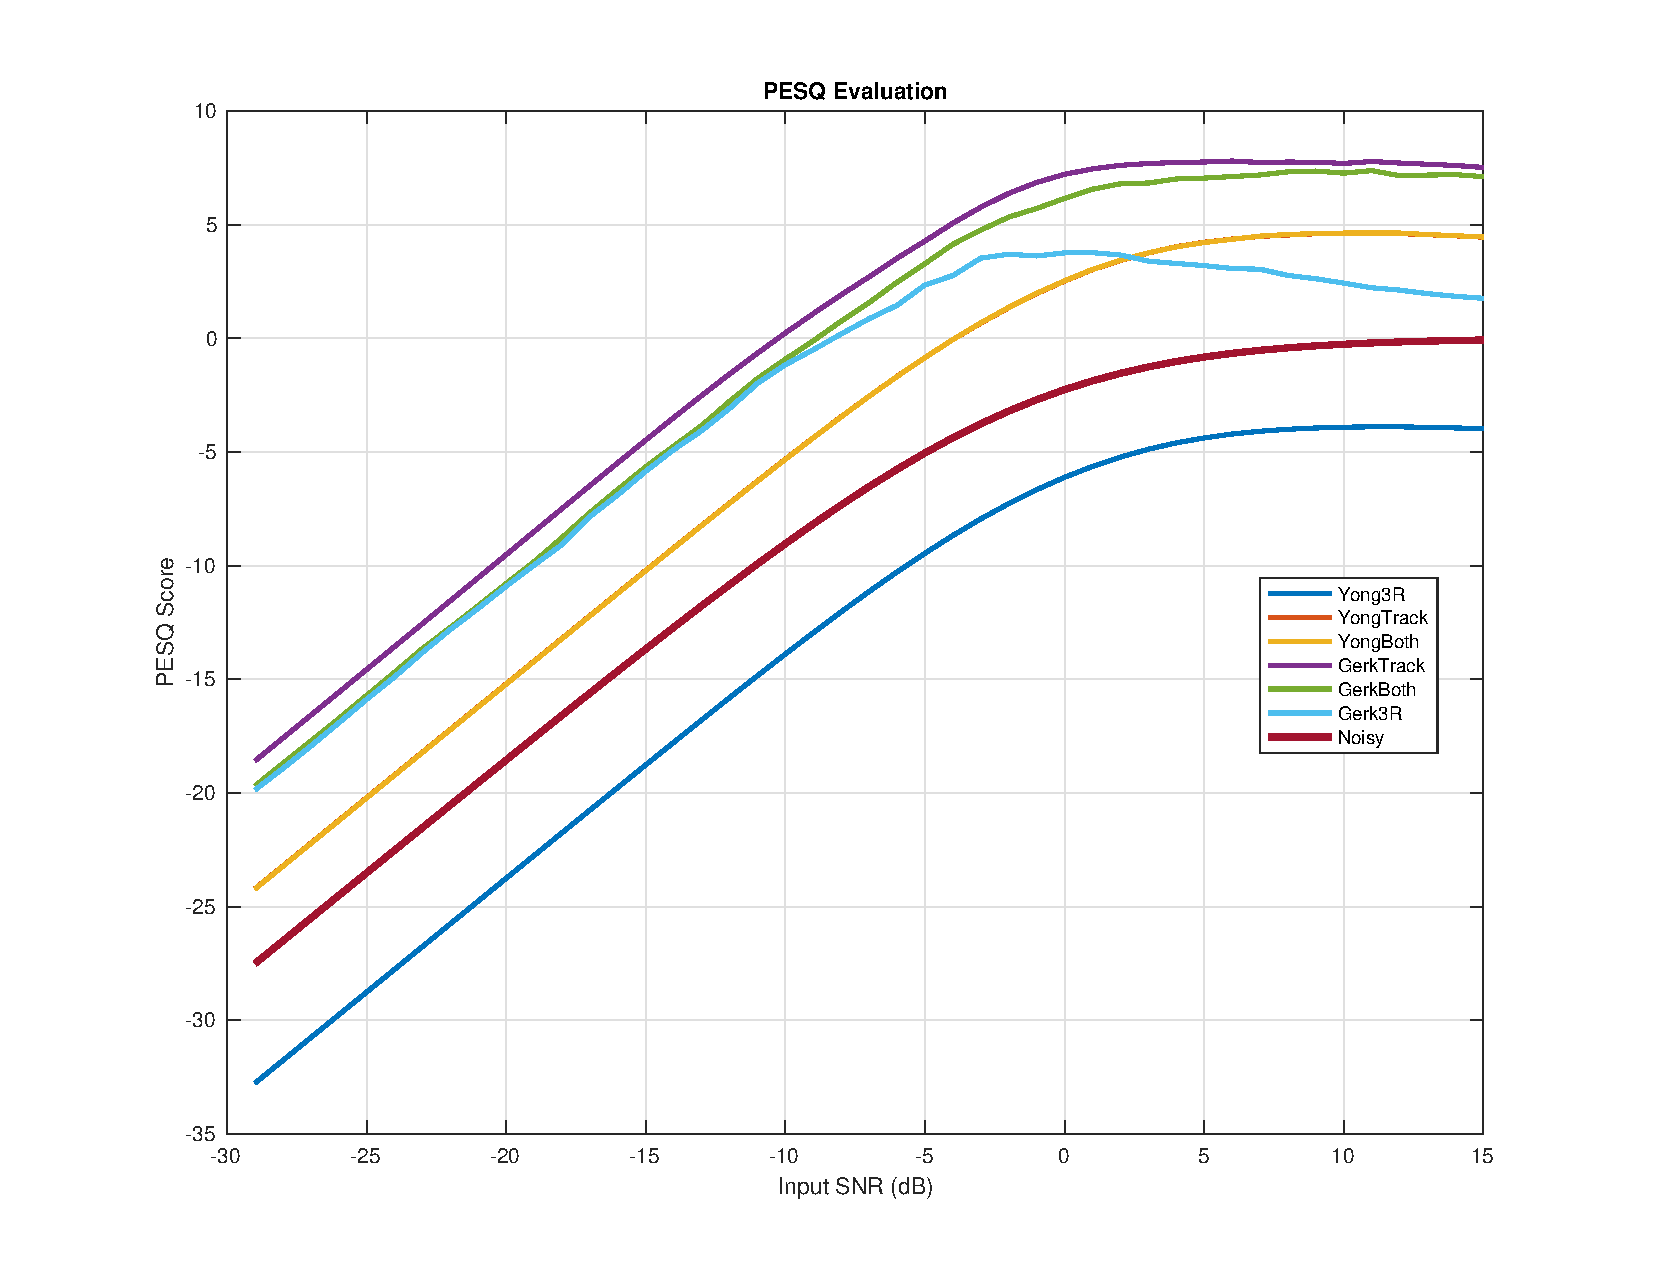
\includegraphics[width=130mm]{Kap4/female2n}
	\caption{PESQ results for female voice and street noise audios.}
	\label{fig:female2n}
\end{figure}

It can also be seen that when the method "Gerk" is combined with the 3 regions algorithm, the performance for low SNR values is always enhancing the speech but when the SNR gets higher, the scores decreases because of speech degradation. The tracking time method can help to fix this, it is shown that this method has high PESQ values for high SNR input values also when mixed with the 3 regions method.\\



\begin{figure}[!ht]
  \centering
	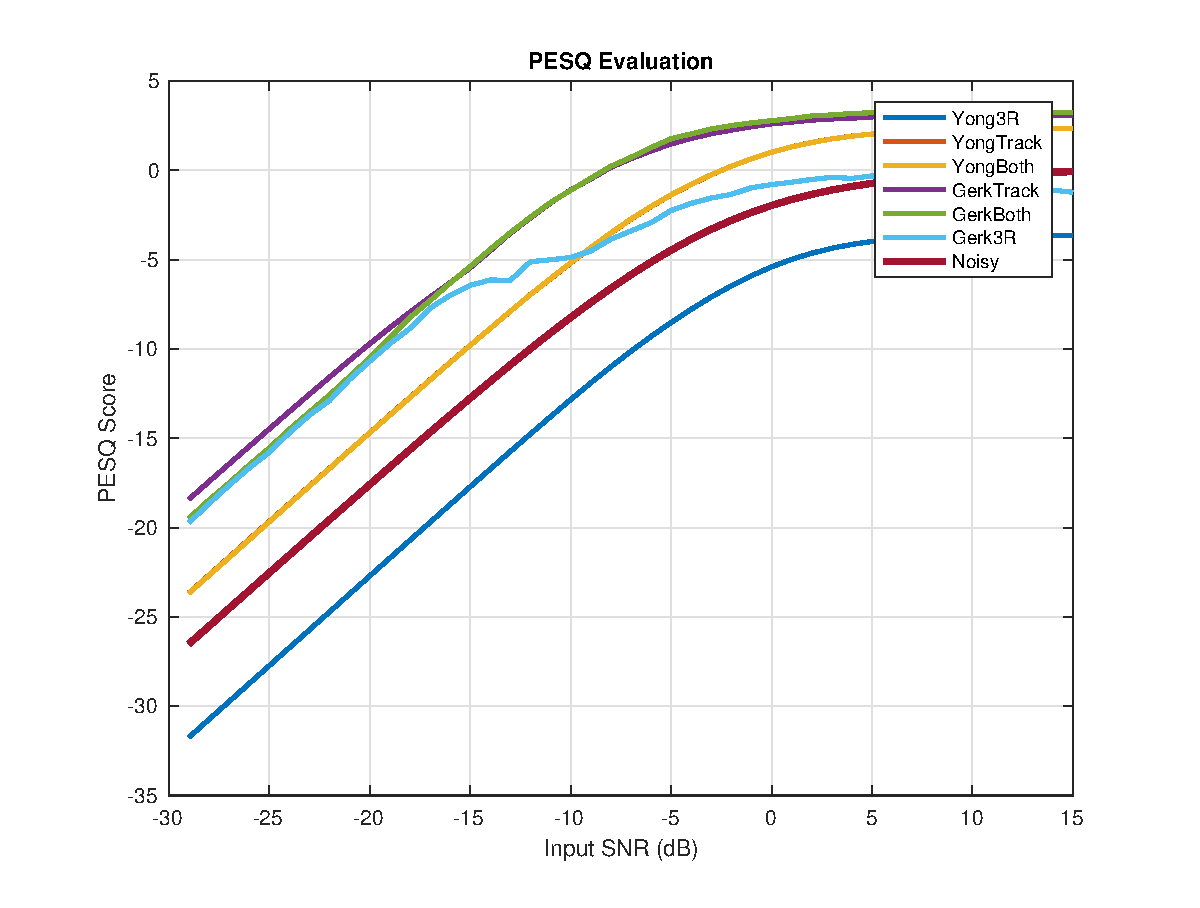
\includegraphics[width=130mm]{Kap4/MaleN1}
	\caption{PESQ results for male voice and street noise audios.}
	\label{fig:MaleN1}
\end{figure}

In general, the method shown in \cite{Gerkmann2011NoisePresence} shows a better performance when being implemented with the MWF. Also it can be noticed that the 3 regions method tends to have better performance for low SNR input values over the tracking time method but this is reversed for higher SNR values. In general, mixing these two algorithms for avoiding stagnation leads to good speech enhancement results. It is just important to notice that the tracking method will have more memory storage.\\

\begin{figure}[!ht]
  \centering
	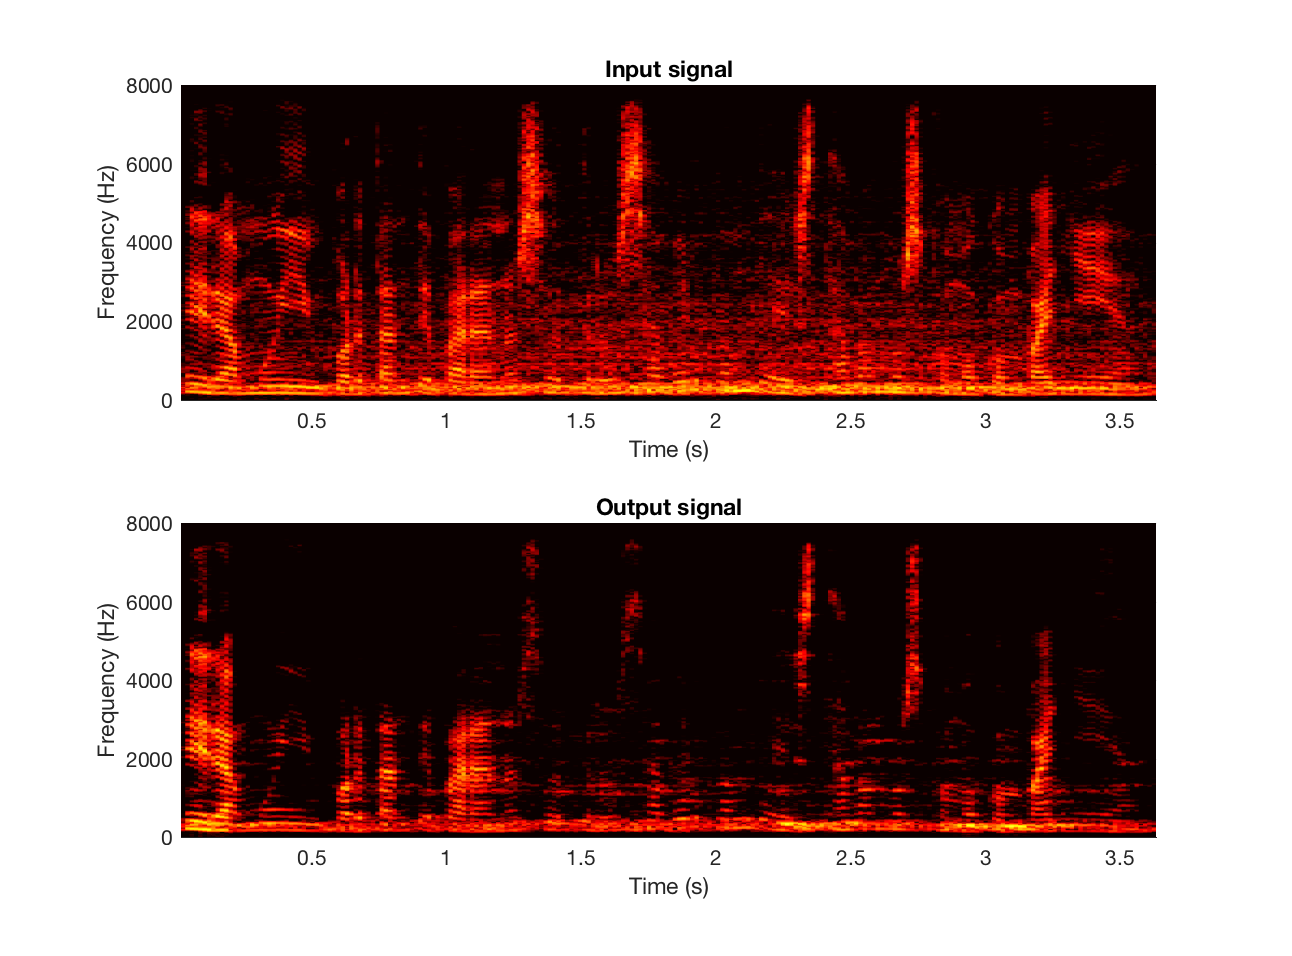
\includegraphics[width=140mm]{Kap4/fil1}
	\caption{Input and out spectrograms when using the MWF with "Gerk" method and both algorithms for avoiding stagnation.}
	\label{fig:fil1}
\end{figure}

In the figure \ref{fig:fil1} is shown the input and output spectogram of one of the test. There it is notorious how big part of the noise is attenuated while preserving the voice. In figure \ref{fig:SPP32} the SPP values of this case are show, it is notorious that there is voice over-estimation (noise taken as voice), but not under-estimation (most of the voice is detected), which is one of the conditions for having a correct reference for the multichannel filter.\\

\begin{figure}[!ht]
  \centering
	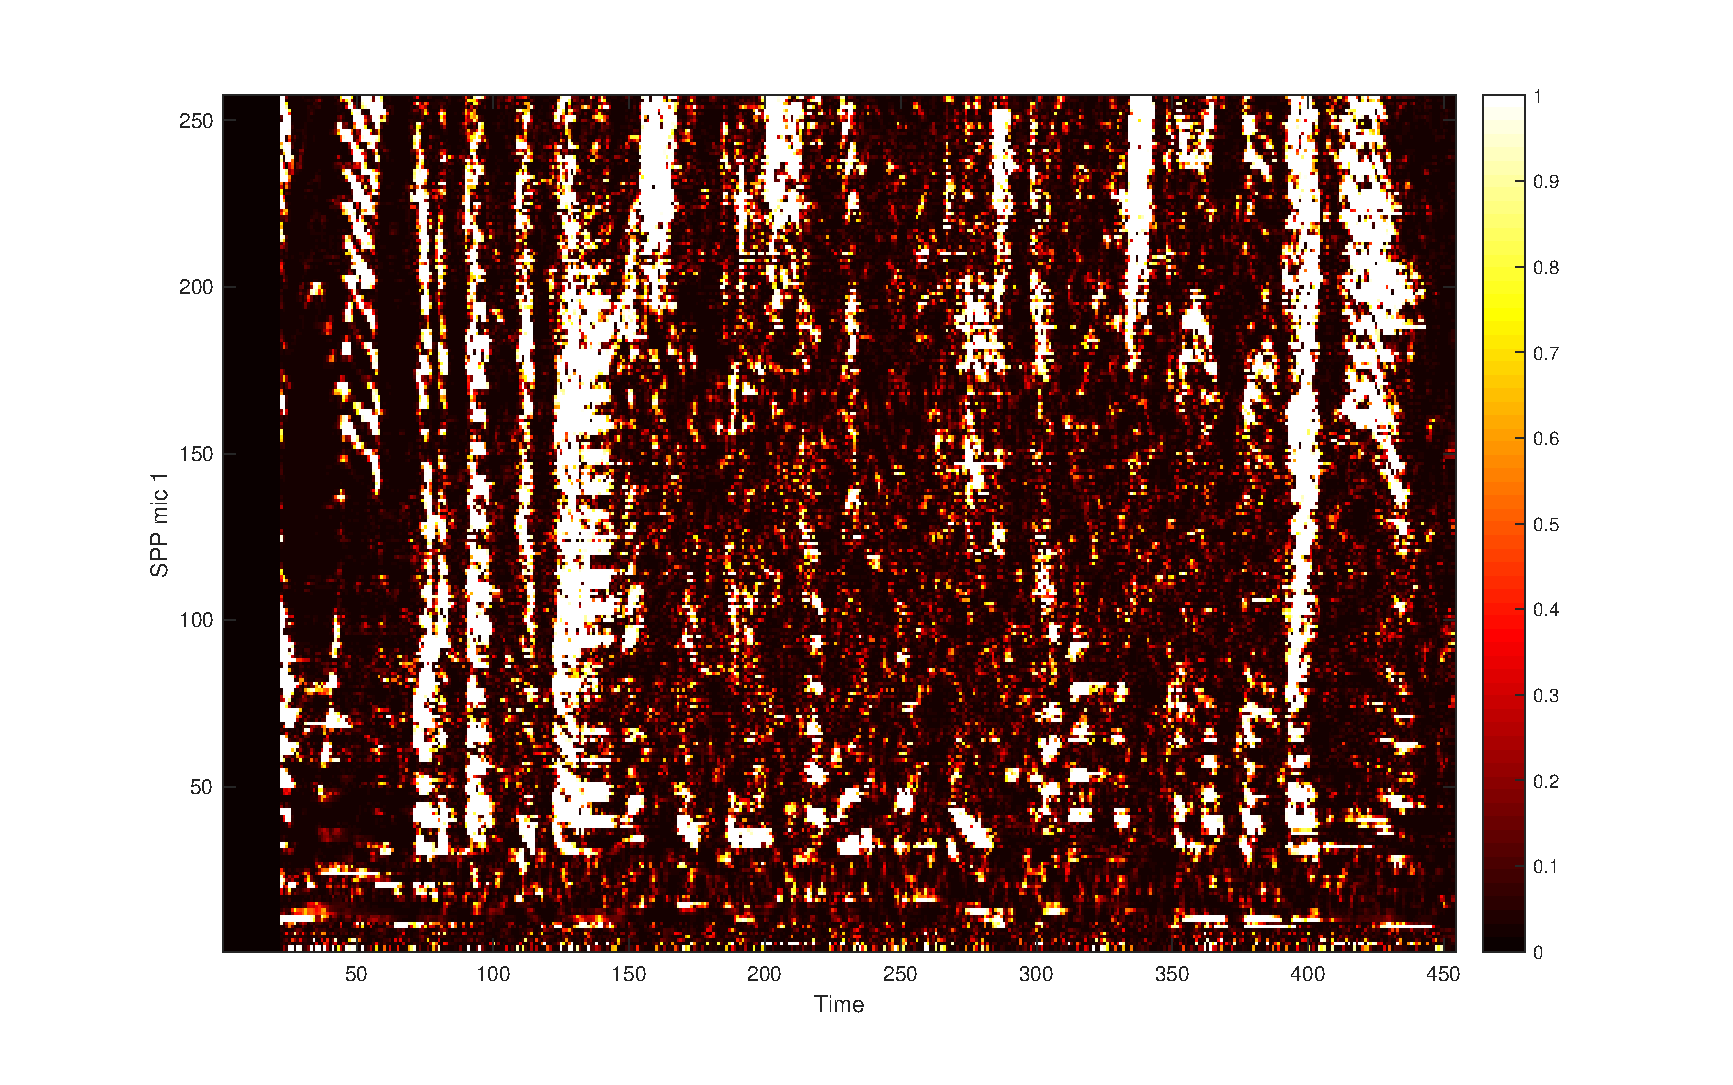
\includegraphics[width=120mm]{Kap4/SPP32}
	\caption{SPP values.}
	\label{fig:SPP32}
\end{figure}





